\section{Différenciation pour la symétrie}

\subsection{Activité des cocottes}\label{annexe:symetrie-act}

Énoncé initial : Chacune des cocottes blanches a été obtenue à partir de la grise par une transformation différente.  Classe les couples de cocottes en fonction des transformations utilisées pour les construire. 

\begin{figure}[h!]
    \centering
    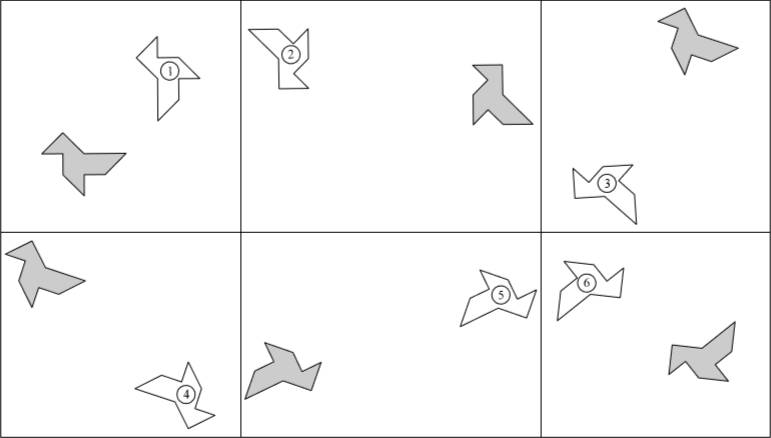
\includegraphics[width=0.9\linewidth]{img/activitemepcc.jpg}
    \caption{Source : \textit{Des maths ensemble et pour chacun 5\up{e}}}
    \label{fig:angles-fiche1}
\end{figure}

\subsection{Fiches méthodologiques}\label{annexe:symetrie-fiches}

Les fiches méthodologiques sont scannées et présentes à cette adresse : \url{https://vvvictoire.github.io/memoire-meef/fiches-methodologiques.html}

\subsection{Activité en salle informatique}\label{annexe:symetrie-tice}

L'analyse complète de la séance est disponible à cette adresse : \url{https://vvvictoire.github.io/memoire-meef/extraits-de-portfolio.html}

\subsection{Analyse d'évaluation portant sur la symétrie}\label{annexe:symetrie-eval}

L'analyse complète de l'évaluation est disponible à cette adresse : \url{https://vvvictoire.github.io/memoire-meef/extraits-de-portfolio.html}

\clearpage

\section{Différenciation pour les angles alternes-internes}

\subsection{Évaluations diagnostiques}\label{annexe:angles-prod1}

Voici quelques citations extraites de copies d'élèves. La question initiale était : 

Les captures d'écran associées à ces citations sont consultables à cette adresse : \url{https://vvvictoire.github.io/memoire-meef/angles-productions-d-eleves.html}

\subsection{Fiches d'exercice}\label{annexe:angles-fiches}

\begin{figure}[h!]
    \centering
    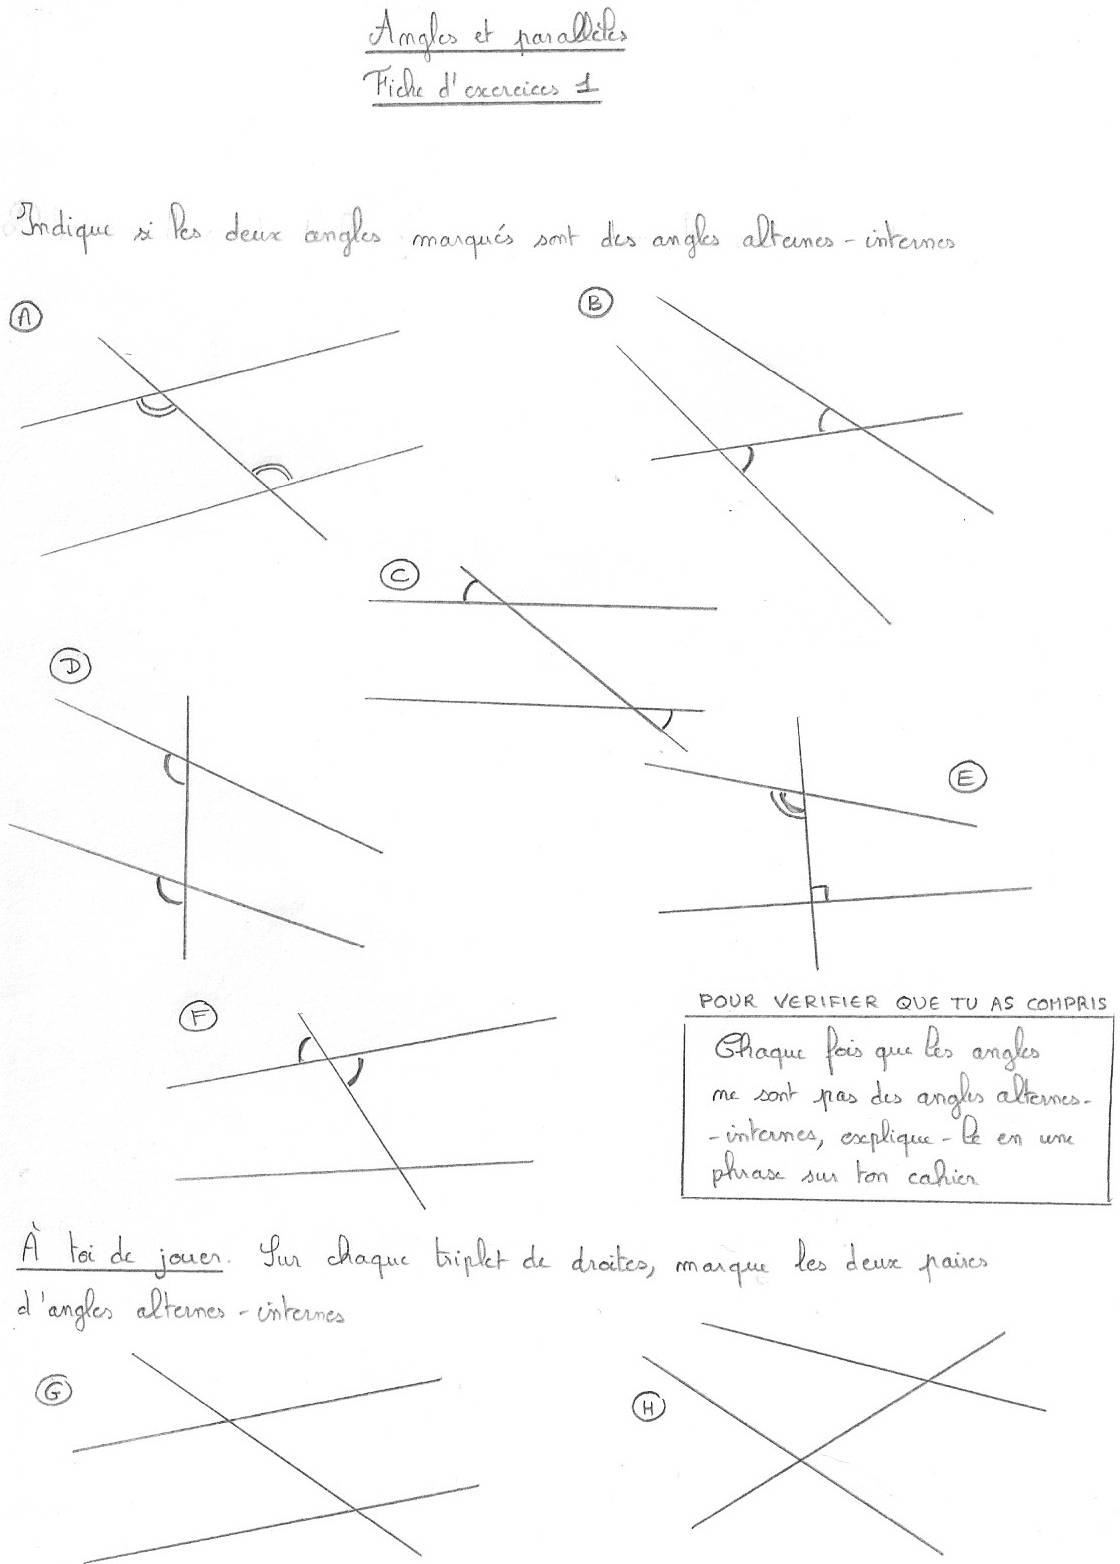
\includegraphics[width=0.6\linewidth]{img/anglesfiche1.jpg}
    \caption{Figure accompagnant les explications destinées à l'enseignant et pouvant être photocopiées et distribuées aux élèves}
    \label{fig:angles-fiche1}
\end{figure}

\begin{figure}[h!]
    \centering
    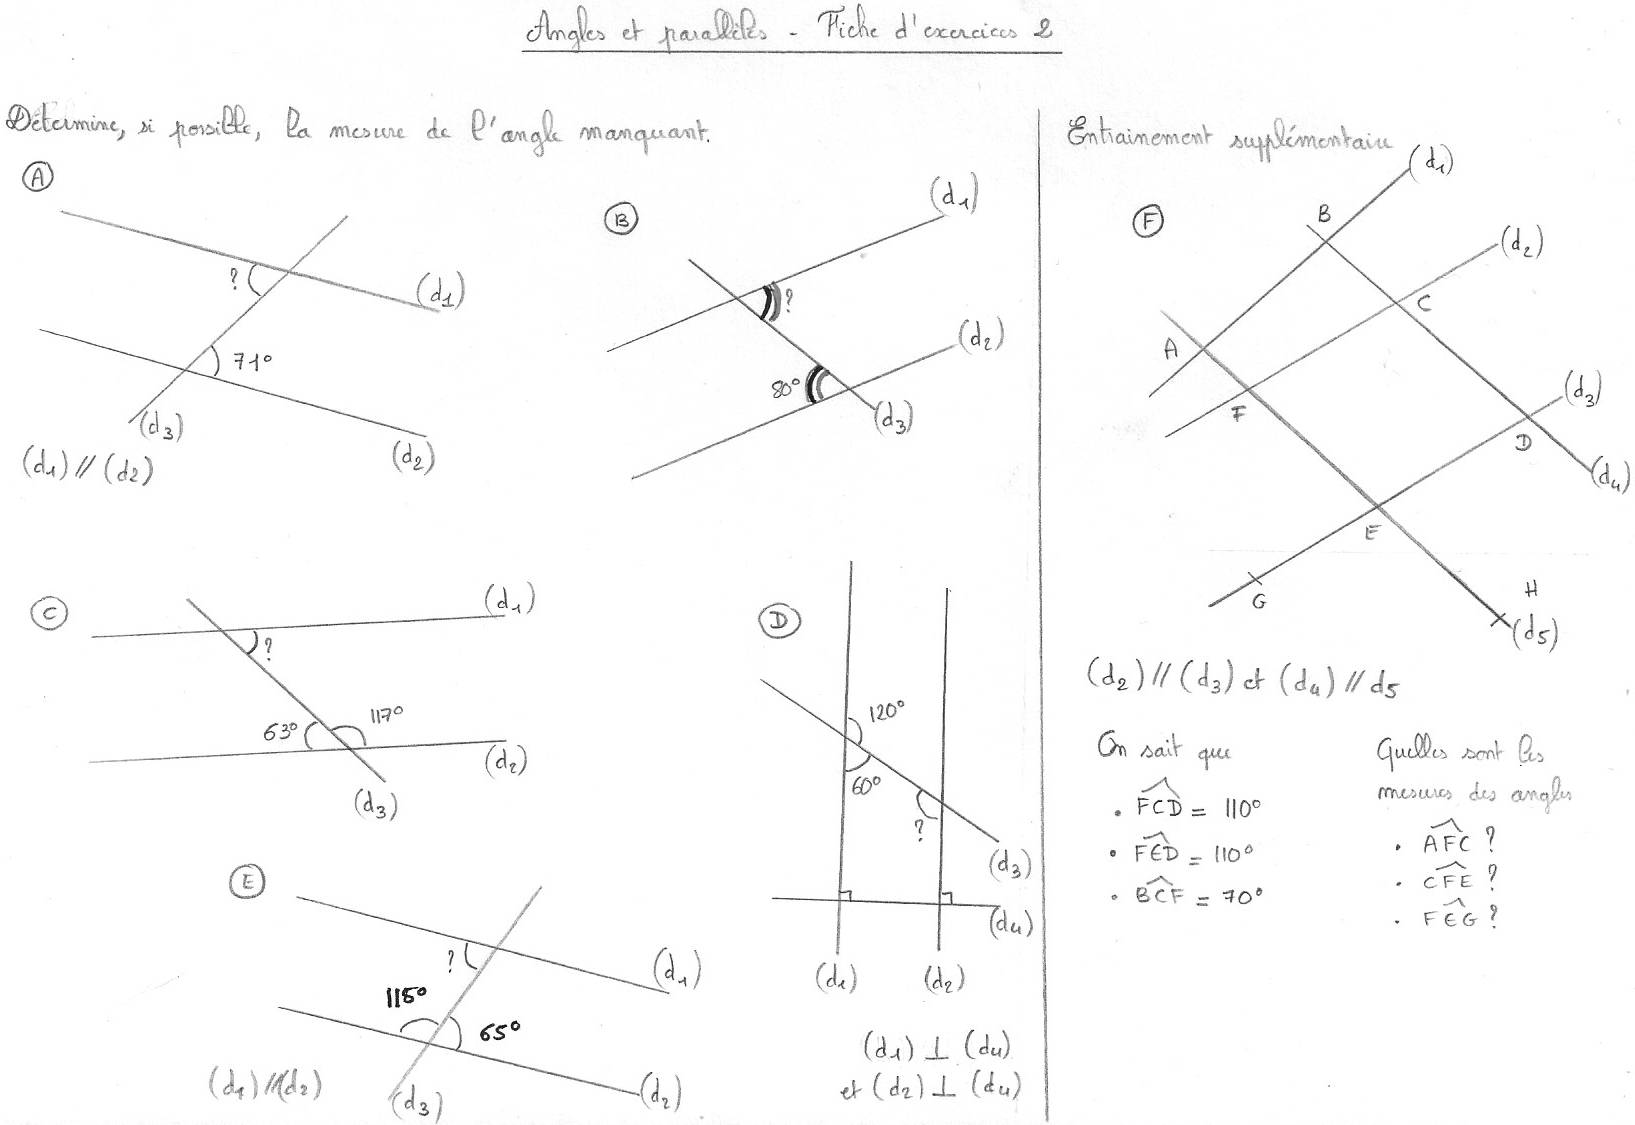
\includegraphics[width=0.8\linewidth]{img/anglesfiche2.jpg}
    \caption{Figure accompagnant les explications destinées à l'enseignant et pouvant être photocopiées et distribuées aux élèves}
    \label{fig:angles-fiche1}
\end{figure}

\begin{figure}[h!]
    \centering
    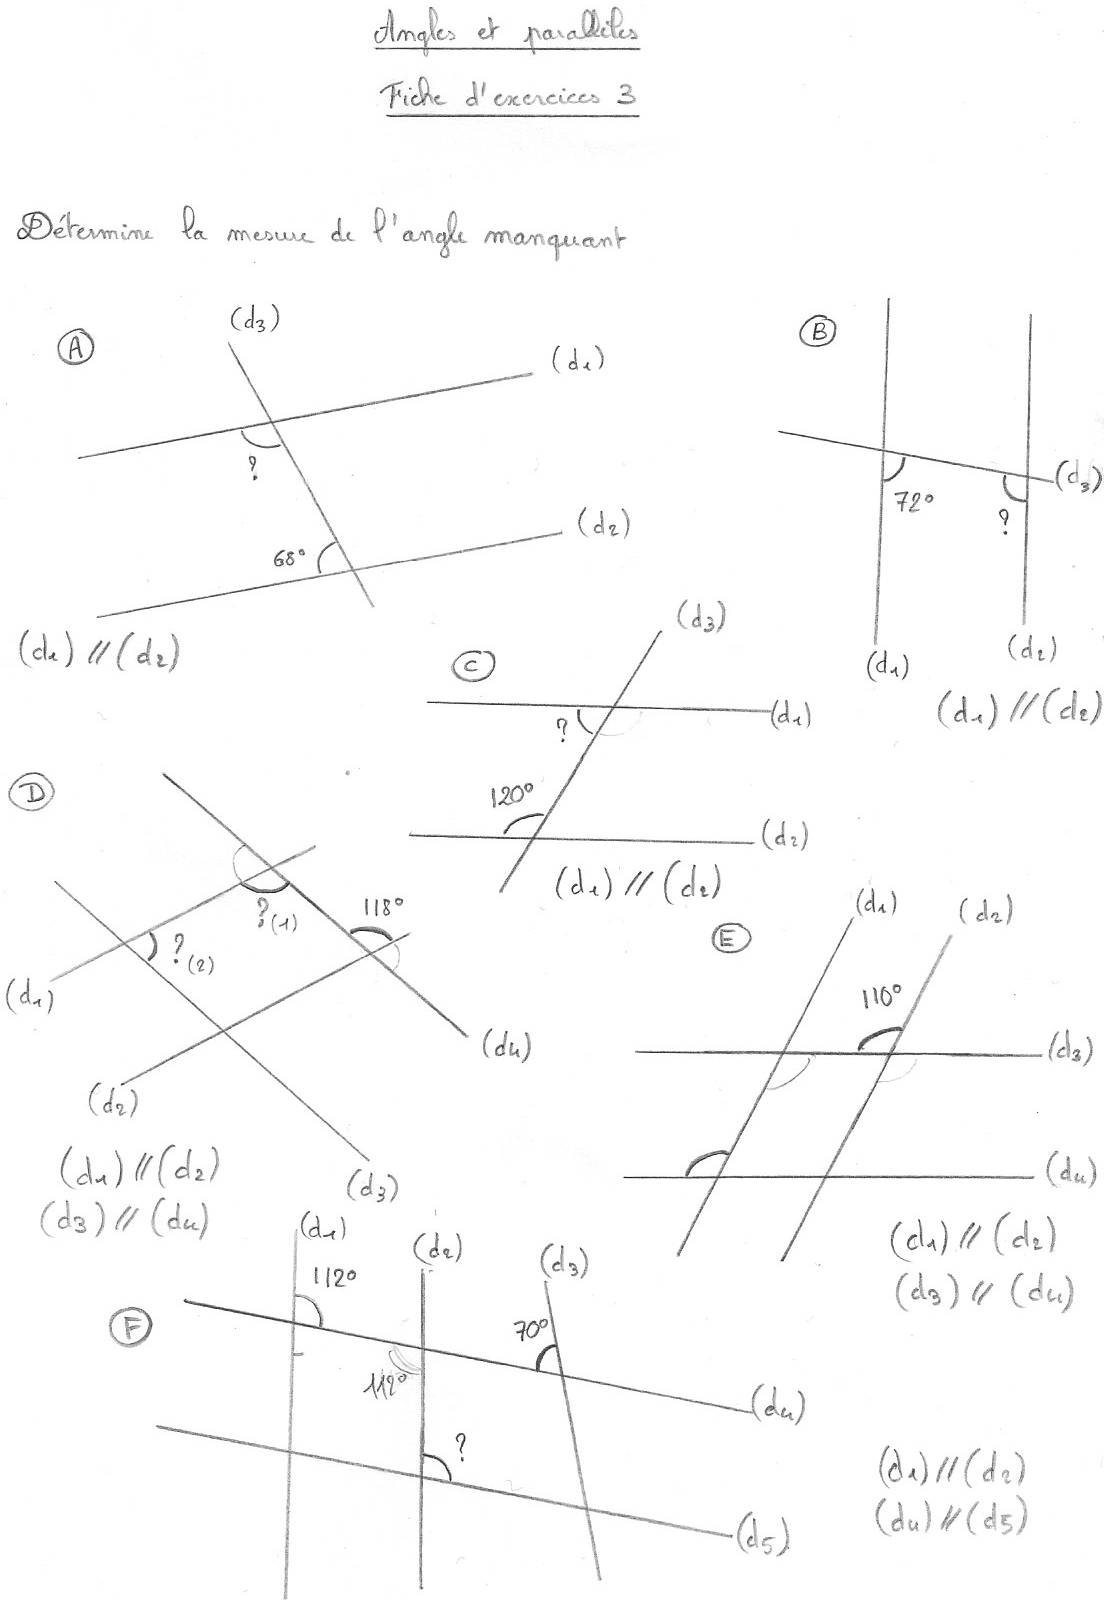
\includegraphics[width=0.6\linewidth]{img/anglesfiche3.jpg}
    \caption{Figure accompagnant les explications destinées à l'enseignant et pouvant être photocopiées et distribuées aux élèves}
    \label{fig:angles-fiche1}
\end{figure}

\clearpage

\subsection{Histoire de la coccinelle et de la libellule}\label{annexe:angles-prod2}

\begin{figure}[h!]
    \centering
    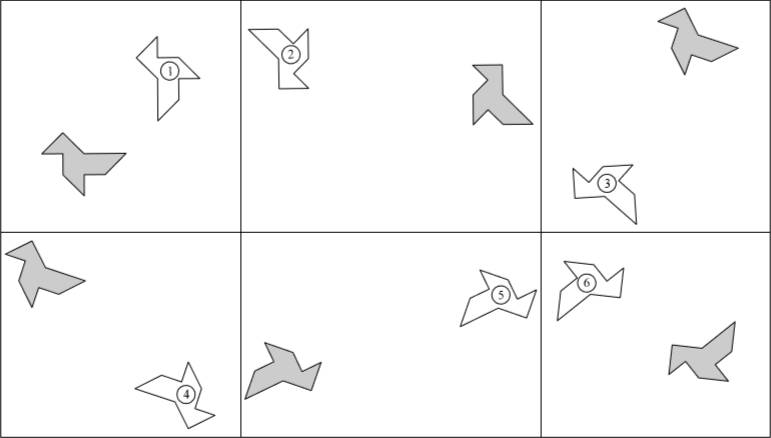
\includegraphics[width=0.9\linewidth]{img/activitemepcc.jpg}
    \caption{Une version où la coccinelle et la libellule sont dessinées.}
    \label{fig:angles-fiche1}
\end{figure}

\begin{figure}[h!]
    \centering
    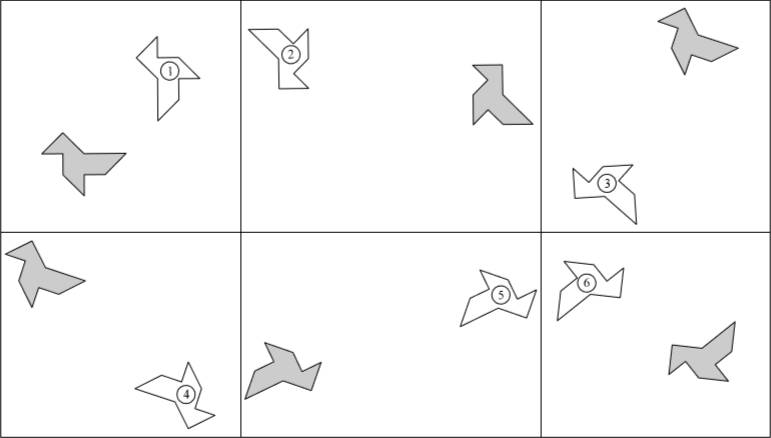
\includegraphics[width=0.9\linewidth]{img/activitemepcc.jpg}
    \caption{Une version évoluée où la coccinelle et la libellule sont schématisées par des points.}
    \label{fig:angles-fiche1}
\end{figure}